%!TEX root = ../main.tex
\chapter{High-Dimensional Linear Regression}
\section{Introduction}
So far we've looked at model selection. For example, we considered the problem of choosing the ``best'' set of regressors for a forecasting problem. Here, the idea was to consider dropping regressors with small coefficients to get a favorable bias-variance tradeoff. There are several problems with this approach. First, variable selection can be unstable because of the discrete nature of the problem: small changes in the underlying data could lead to large changes in the selected set of regressors. Second, it is only computationally infeasible to consider all possible subsets of regressors when $p < 30$. Our colleague Andy Postelwaite actually has a microeconomic theory paper about this called ``Fact Free Learning.'' You should check it out: it's very interesting!

In this lecture we'll consider an alternative to model selection called ``shrinkage.'' The idea is roughly as follows: rather than making a discrete choice of which variables are ``in'' and which are ``out,'' it might make more sense to leave everything in the model but ``regularize'' or ``shrink'' the estimated coefficients away from the maximum likelihood estimator, much as a Bayesian prior does. Rather than attempting to incorporate prior beliefs, however, here the idea is merely to find a clever way of adding bias that buys us a large decrease in variance. There will still be a model selection component here, but it will involve a single, continuous ``tuning'' or ``smoothing'' parameter.

\section{References}
Some good references for the material discussed here are Hastie, Tibshirani \& Friedman (2008; Chapter 3), and Murphy (2012; Chapters 7 \& 13). I'll also refer to some specifid papers which I'll post on Canvas.

\section{Review of Matrix Decompositions}
\subsection{The QR Decomposition}
Any $n\times k$ matrix $A$ with full column rank can be decomposed as $A = QR$, where $R$ is an $k\times k$ upper triangular matrix and $Q$ is an $n\times k$ matrix with orthonormal columns. The columns of $A$ are \emph{orthogonalized} in $Q$ via the Gram-Schmidt process. Since $Q$ has orthogonal columns, we have $Q'Q = I_k$. It is \emph{not} in general true that $QQ' = I$, however. In the special case where $A$ is square, $Q^{-1} = Q'$.

\paragraph{Note:} The way we have defined things here is here is sometimes called the ``thin'' or ``economical'' form of the QR decomposition, e.g.\ \texttt{qr\_econ} in Armadillo. In our ``thin'' version, $Q$ is an $n\times k$ matrix with orthogonal columns. In the ``thick'' version, $Q$ is an $n\times n$ \emph{orthogonal} matrix. Let $A = QR$ be the ``thick'' version and $A = Q_1 R_1$ be the ``thin'' version. The connection between the two is as follows:
  $$A = QR = Q \left[\begin{array}
    {c} R_1 \\ 0 
  \end{array} \right] = \left[  \begin{array}
    {cc} Q_1 & Q_2
  \end{array}\right]\left[\begin{array}
    {c} R_1 \\ 0 
  \end{array} \right] = Q_1 R_1$$

\paragraph{Least-Squares via the QR Decomposition} We can calculate the least squares estimator of $\beta$ as follows
\begin{eqnarray*}
  \widehat{\beta} &=& (X'X)^{-1} X'y = \left[(QR)' (QR) \right]^{-1} (QR)' y\\
    &=&\left[ R' Q' Q R\right]^{-1} R'Q' y = (R'R)^{-1} R'Q y\\
    &=& R^{-1} (R')^{-1} R' Q'y = R^{-1} Q'y
\end{eqnarray*}
In other words, $\widehat{\beta}$ is the solution to $R\beta = Q'y$. While it may not be immediately apparent, this is a much easier system to solve that the normal equations $(X'X) \beta = X'y$. Because $R$ is \emph{upper triangular} we can solve $R\beta = Q'y$ extremely quickly. The product $Q'y$ is a vector, call it $v$, so the system is simply
  $$\left[
    \begin{array}
      {cccccc}
      r_{11} & r_{12}  & r_{13}& \cdots & r_{1,n-1} & r_{1k} \\
      0 & r_{22} & r_{23}&\cdots & r_{2,n-1} & r_{2k}\\
      0&  0 &  r_{33}& \cdots & r_{3,n-1} & r_{3k}\\  
      \vdots & \vdots & \ddots& \ddots & \vdots & \vdots\\
      0 & 0 & \cdots &0  & r_{k-1, k-1} & r_{k-1, k} \\
      0 & 0 & \cdots & 0 & 0 & r_{k}
    \end{array}
  \right] \left[ \begin{array}
    {ccc}
    \beta_1 \\ \beta_2 \\ \beta_3 \\ \vdots \\ \beta_{k-1} \\ \beta_k
  \end{array}\right] = \left[ \begin{array}
    {c}
    v_1  \\ v_2  \\ v_3 \\  \vdots \\ v_{k-1} \\ v_{k}
  \end{array}\right]
  $$
Hence, $\beta_k = v_k / r_k$ which we can substitute into $\beta_{k-1} r_{k-1,k-1} + \beta_k r_{k-1,k} = v_{k-1}$ to solve for $\beta_{k-1}$, and so on. This is called \textbf{back substitution}. We can use the same idea when a matrix is \emph{lower triangular} only in reverse: this is called \textbf{forward substitution}.

To calculate the variance matrix $\sigma^2 (X'X)^{-1}$ for the least-squares estimator, simply note from the derivation above that $(X'X)^{-1} = R^{-1} (R^{-1})'$ . Inverting $R$, however, is easy: we simply apply back-substitution \emph{repeatedly}. Let $A$ be the inverse of $R$, $\mathbf{a}_j$ be the $j$th column of $A$, and $\mathbf{e}_j$ be the $j$th element of the $k\times k$ identity matrix, i.e.\ the $j$th standard basis vector. Inverting $R$ is equivalent to solving $R \mathbf{a}_1 = \mathbf{e}_1$, followed by $R \mathbf{a}_2 = \mathbf{e}_2$, and so on all the way up to $R \mathbf{a}_k = \mathbf{e}_k$. In Armadillo, if you enclose a matrix in \texttt{trimatu()} or \texttt{trimatl()}, and then request the inverse, the library will carry out backward or forward substitution, respectively.

\paragraph{Othogonal Projection Matrices and the QR Decomposition}
Consider a projection matrix $P_X = X (X'X)^{-1}X'$. Provided that $X$ has full column rank, we have
begin
  $$P_X  = QR(R'R)^{-1}R'Q' = QRR^{-1} (R')^{-1}R'Q' = QQ'$$
Recall that, in general, it is \emph{not} true that $QQ' = I$ even though $Q'Q = I$ because we're using the \emph{economical} QR decomposition in which $Q$ has orthonormal columns but may not be a square matrix. Just to make this completely transparent, consider a very simple example:
	$$X = \left[ \begin{array}
		{cc} 1 & 0 \\ 0 & 1 \\ 0 & 0
	\end{array}\right]$$
Then, we have
	$$X'X = \left[\begin{array}
		{ccc} 1& 0 & 0 \\ 0 & 1 & 0
	\end{array} \right]\left[ \begin{array}
		{cc} 1 & 0 \\ 0 & 1 \\ 0 & 0
	\end{array}\right] = \left[\begin{array}
		{cc} 1 & 0 \\ 0 & 1
	\end{array} \right]$$
but 
	$$XX' = \left[ \begin{array}
		{cc} 1 & 0 \\ 0 & 1 \\ 0 & 0
	\end{array}\right]\left[\begin{array}
		{ccc} 1& 0 & 0 \\ 0 & 1 & 0
	\end{array} \right] = \left[\begin{array}
		{ccc} 1 & 0 & 0 \\ 0 & 1 & 0 \\ 0 & 0 & 0
	\end{array} \right]$$
It's important to keep the fact that $UU' \neq I$ in mind when using the QR decomposition for more complicated matrix calculations.

\subsection{The Singular Value Decomposition}
The Singular Value Decomposition (SVD) is probably the most elegant result in linear algebra. It's also an invaluable computational and theoretical tool in statistics and econometrics. I can only give a brief overview here, but I'd encourage you to learn more when you have time. Some excellent references are Strang (1993) and Kalman (2002).

\paragraph{The SVD} Any $m \times n$ matrix $A$ of arbitrary rank $r$ can be decomposed according to 
	$$X = UDV' = (\mbox{orthogonal})(\mbox{diagonal})(\mbox{orthogonal})$$
	\begin{itemize}
	 	\item $U$ is an $m\times m$ orthogonal matrix whose columns contain the eigenvectors of $AA'$
	 	\item $V$ is an $n\times n$ orthogonal matrix whose columns contain the eigenvectors of $A'A$
	 	\item $D$ is an $m\times n$ matrix whose first $r$ main diagonal elements are the  \emph{singular values} $d_1, \hdots, d_r$. All other elements of $D$ are zero.
	 	\item The singular values $d_1, \hdots, d_r$ are the positive eigenvalues of $A'A$ which are \emph{identical} to the positive eigenvalues of $AA'$.
	 \end{itemize} 

\paragraph{The Four Fundamental Subspaces} It turns out that the SVD provides orthonormal bases for each of the so-called ``fundamental subspaces'' of a matrix $A$. In particular:
	\begin{enumerate}
		\item \textbf{column space}: first $r$ columns of $U$
		\item \textbf{row space}: first $r$ columns of $V$
		\item \textbf{null space}: last $n - r$ columns of $V$
		\item \textbf{left null space}: last $m - r$ columns of $U$
	\end{enumerate}

\paragraph{SVD for Symmetric Matrices} If $A$ is symmetric then, by the spectral theorem, we can write $A = Q\Lambda Q'$ where $\Lambda$ is a diagonal matrix containing the eigenvalues of $A$ and $Q$ is an orthonormal matrix whose columns are the corresponding eigenvectors. In this case, $U = V = Q$ and $D$ is simply the absolute value of $\Lambda$ (i.e.\ negative eigenvalues become positive singular values).

\paragraph{SVD for Positive Definite Matrices} If $A$ is not only symmetric but \emph{positive definite}, then $A = Q\Lambda Q'$ is the \emph{same decomposition} as $A = UDV'$: $U=V=Q$ and $\Lambda = D$.

\paragraph{The ``Economical'' SVD}
The number of singular values equals $r$, the rank of $A$, which is at most $\max\{m,n\}$. This means that some of the columns of $U$ or $V$ will be \emph{irrelevant} since they will be multiplied by zeros in $D$. Accordingly, most linear algebra libraries provide an ``economical'' SVD that only calculate the columns of $U$ and $V$ that are multiplied by non-zero values in $D$. In Armadillo, for example, the command is \texttt{svd\_econ}. 

We can write the economical SVD in summation form as 
	$$A = \sum_{i=1}^r d_i \textbf{u}_i \textbf{v}_i'$$
where $r = \mbox{rank}(A)$ and the singular values $d_i$ are arranged in order from largest to smallest. In matrix form, this is given by:
	$$\underset{(n\times p)}{A} = \underset{(n\times r)}{U} \underset{(r\times r)}{D} \underset{(r\times p)}{V'}$$
In the economical SVD, $U$ and $V$ may no longer be square, so they are not orthogonal matrices but their \emph{columns} are still orthonormal.

\paragraph{Approximation Property of SVD} The Frobenius norm of a matrix $A$ is given by
	$$||A||_F = \sqrt{\sum_{i=1}^m \sum_{i=1}^n a_{ij}^2} = \sqrt{\mbox{trace}(A'A)}$$
Using this norm as a measure of ``approximation error'', it can be shown that the SVD provides the \emph{best low rank approximation} to a matrix $X$. 

Using the ``economical'' form of the SVD, we can write
	$$X = \sum_{i=1}^r d_i \textbf{u}_i \textbf{v}_i'$$
where the index is $i$ is defined such that the \emph{largest} singular value comes first, followed by the second largest, and so on. This expression gives the rank-$r$ matrix $X$ as a \emph{sum} of $r$ rank-1 matrices. Now suppose that the rank of $X$ is large and we wanted to \emph{approximate} $X$ using a matrix $\widehat{X}_L$ with rank $L<k$. If we measure the reconstruction error using the Frobenius norm, it can be shown that the \emph{truncated SVD}
	$$\widehat{X}_L = \sum_{i=1}^{L} d_i \textbf{u}_i \textbf{v}_i'$$ 	
provides the best rank $L$ approximation to $X$. In other words, $\widehat{X}_L$ is the $\arg \min$  over all rank $L$ matrices of the quantity $||X - \widehat{X}_L||_F$. It is also possible to provide bounds on the quality of the approximation, and thus choose an appropriate truncation. 

\section{Gauss-Markov, meet James-Stein}
Consider the linear regression model
	$$\mathbf{y} = X\beta + \boldsymbol{\epsilon}$$
In Econ 705 you learned that ordinary least squares (OLS) is the minimum variance unbiased linear estimator of $\beta$ under the assumptions $E[\boldsymbol{\epsilon}|X] = \mathbf{0}$ and $Var(\mathbf{\epsilon}|X) = \sigma^2 I$. When the second assumption fails, you learned that generalized least squares (GLS) provides a lower variance estimator than OLS. All of this is fine, as far as it goes, but there's an obvious objection: why are we restricting ourselves to unbiased estimators? Generically, we know that there is a bias-variance tradeoff. So what happens if we allow ourselves to consider biased estimators? 



\subsection{Dominance and Admissibility}
To understand what follows, we'll need two concepts from decision theory: \textbf{dominance} and \emph{admissibility}. Let $\widehat{\theta}$ and $\widetilde{\theta}$ be two estimators of $\theta$, and $R$ be a risk function, e.g.\ MSE. We say that $\widehat{\theta}$ \textbf{dominates} $\widetilde{\theta}$ with respect to $R$ if $R(\widehat{\theta},\theta) \leq R(\widetilde{\theta},\theta)$ for \emph{all} possible values of $\theta$ wand the inequality is \emph{strict} for \emph{at least one} possible value of $\theta$. We say that $\widehat{\theta}$ is \textbf{admissible} if there is no estimator that dominates it. To prove that an estimator is \textbf{inadmissible} it suffices to find an estimator that dominates it.

\subsection{The James-Stein Estimator}
It turns out that OLS is inadmissible relative to MSE loss when $p\geq 3$. This result was so surprising when first discovered that it is sometimes called ``Stein's Paradox.'' Efron and Morris (1977) provide a nice discussion. An estimator that can be shown to dominate OLS is the so-called ``positive-part James-Stein estimator'' which is given by
	$$\widehat{\beta}^{JS} = \widehat{\beta}\left[1 -\frac{(p-2)\sigma^2}{\widehat{\beta}' \widehat{\beta}} \right]_+$$
where $\widehat{\beta}$ is the OLS estimator and $(x)_+ = \max(x,0)$. To make this operational, we substitute an estimator of $\sigma^2$, for example one based on the OLS residuals. We see that this estimator shrinks us \emph{away} from the least-squares fit and towards zero. 

Since James-Stein beats OLS, we know that shrinkage is a good idea. Now we'll consider some more general forms of shrinkage, starting with Ridge Regression.



\section{Ridge Regression} 
Ridge regression is a technique that was originally designed to address the problem of multicollinearity. When two or more predictors are very strongly correlated, OLS can become unstable. For example, if $x_1$ and $x_2$ are \emph{nearly} linearly dependent, a large positive coefficient $\beta_1$ could effectively \emph{cancel out} a large negative coefficient $\beta_2$. Ridge Regression attempts to solve this problem by \emph{shrinking the estimated coefficients towards zero and towards each other}. This is accomplished by adding a squared $L_2$-norm ``penalty'' to the OLS objective function, yielding
	$$\widehat{\beta}_{Ridge} =\underset{\beta}{\arg \min} (\mathbf{y} - \textbf{1}_n\beta_0 - X\beta)' (\mathbf{y} - \textbf{1}_n \beta_0 - X\beta) + \lambda \beta'\beta$$
where $\textbf{1}_n$ is an $(n\times 1)$ vector of ones, $\beta_0$ denotes the regression intercept and $\beta = (\beta_1, \hdots, \beta_p)'$ the remaining coefficients. The Ridge Penalty parameter $\lambda$ is a non-negative constant that we have to choose. Note that we do \emph{not} penalize the intercept in Ridge Regression. The easiest and most common way to handle this is simply to de-mean both $X$ and $\mathbf{y}$ before proceeding. so that there is no intercept and the problem becomes
	$$\widehat{\beta}_{Ridge} =\underset{\beta}{\arg \min}(\mathbf{y} - X\beta)' (\mathbf{y} - X\beta) + \lambda \beta'\beta$$
Throughout these notes we will assume that everything has been de-meaned so there is no intercept.

\subsection{Ridge is \emph{Not} Scale Invariant} When we carry out OLS, if we re-scale a regressor $\mathbf{x}$, replacing it with $c \mathbf{x}$ where $c$ is some nonzero constant, then the corresponding OLS coefficient estimate is scaled by $1/c$ to compensate. In other words, OLS is \emph{scale invariant}. The same is not true of Ridge Regression, so it is common to convert the columns of the design matrix to the same units before proceeding. The usual way of handling this is simply to \emph{standardize} each of the regressors.

\subsection{Another Way to Express Ridge Regression}
The following is an equivalent statement of the Ridge Regression problem:
$$\widehat{\beta}_{Ridge} = \underset{\beta}{\arg \min}(\mathbf{y} - X\beta)' (\mathbf{y} - X\beta) \quad \mbox{subject to} \quad \beta'\beta \leq t$$
In other words, Ridge Regression is like least squares ``on a budget.'' If you want to make one coefficient estimate larger, you have to make another one smaller. The ``income'' level $t$ maps one-to-one to $\lambda$, although the mapping is data-dependent.

\subsection{Ridge as Bayesian Linear Regression}
As you may recall from the first part of the semester, Bayesian models with informative priors automatically provide a form of shrinkage. Indeed, many frequentist shrinkage estimators can be expressed in Bayesian terms. Provided that we ignore the regression constant, the solution to Ridge Regression is \emph{equivalent} to MAP (maximum a posteriori) estimation based on the following  Bayesian regression model
	\begin{eqnarray*}
		y|X, \beta, \sigma^2 &\sim& N(X\beta,\sigma^2 I_n) \\
		\beta &\sim& N(\mathbf{0}, \tau^2 I_p)
	\end{eqnarray*}
where $\sigma^2$ is assumed known and $\lambda = \sigma^2/\tau^2$. In other words, Ridge Regression gives the \textbf{posterior mode}. Since this model is conjugate, the posterior is normal. Thus, in addition to being the MAP estimator, the solution to Ridge Regression is also the posterior mean.


\subsection{An Explicit Formula for Ridge Regression}
The objective function is
\begin{eqnarray*}
	Q_{ridge}&=& (\mathbf{y} - X\beta)' (\mathbf{y} - X\beta) + \lambda \beta'\beta\\
	&=&\mathbf{y}'\mathbf{y} - \beta'X \mathbf{y} - \mathbf{y}'X\beta + \beta'X'X \beta + \lambda \beta' I_p \beta\\
	&=& \mathbf{y}'\mathbf{y} - 2 \mathbf{y}'X\beta + \beta'(X'X + \lambda I_p)\beta
\end{eqnarray*}
Recall the following facts about matrix differentiation\footnote{See, for example, Harville (1997; Chapter 15).}
	\begin{eqnarray*}
		\frac{\partial (\mathbf{a}' \mathbf{x})}{\partial \mathbf{x}}  &=& \mathbf{a}\\
		\frac{\partial( \mathbf{x}'A \mathbf{x})}{\partial \mathbf{x}} &=& (A + A')\mathbf{x}
	\end{eqnarray*}
Thus, we have 
$$\frac{\partial}{\partial \beta} Q(\beta) = -2X'\bf{y} + 2(X'X + \lambda I_p)\beta$$
since $(X'X + \lambda I_p)$ is symmetric. Thus, the first order condition is 
	$$X'\textbf{y} = (X'X + \lambda I_p)\beta$$
Hence,
	$$\widehat{\beta}_{Ridge} = (X'X + \lambda I_p)^{-1} X'\textbf{y}$$
So is $(X'X + \lambda I_p)$ guaranteed to be invertible? We need this to be the case for the solution of the Ridge Regression problem to be unique. In the following section, we'll provide an alternative way of analyzing the problem by turning it into something we're more familiar with: OLS.

\subsection{Ridge Regression via OLS}
From the first half of the semester, you may recall that Bayesian linear regression can be thought of as ``plain-vanilla'' OLS using a design matrix that has been \emph{augemented} with ``fake'' observations that represent the prior. This turns out to be a very helpful way of looking at Ridge Regression. Define

$$\widetilde{\textbf{y}} = \left[ \begin{array}
	{c} \textbf{y} \\ \textbf{0}_p
\end{array}\right], \quad \quad \widetilde{X} = \left[ \begin{array}
	{c} X \\ \sqrt{\lambda} I_p
\end{array}\right]$$
The objective function for Ridge Rgression is \emph{identical} to the OLS objective function for the augmented dataset, namely
	$$\underset{\beta}{\arg \min} \left(\widetilde{\mathbf{y}} - \widetilde{X}\beta\right)'\left(\widetilde{\mathbf{y}} - \widetilde{X}\beta\right)$$
Which we can show as follows:
\begin{eqnarray*}
	\left(\widetilde{\mathbf{y}} - \widetilde{X}\beta\right)'\left(\widetilde{\mathbf{y}} - \widetilde{X}\beta\right) &=& \left[\begin{array}
		{cc} (\mathbf{y} - X\beta)' & (-\sqrt{\lambda}\beta)'
	\end{array} \right] \left[\begin{array}
		{c} (\mathbf{y} - X\beta) \\ -\sqrt{\lambda} \beta
	\end{array} \right]\\
		&=& (\mathbf{y} - X\beta)' (\mathbf{y} - X\beta) + \lambda \beta'\beta\\
\end{eqnarray*}

\subsection{Ridge is Always Unique} We know that the OLS estimator is only unique provided that the design matrix has full column rank. In constrast there is \emph{always} a unique solution to the Ridge Regression problem, even when there are more regressors than observations. This follows \emph{immediately} from the preceding: the columns of $\sqrt{\lambda}I_p$ are linearly independent, so the columns of the augmented data matrix $\widetilde{X}$ are \emph{also} linearly independent, \emph{regardless} of whether the same holds for the columns of $X$. Thus we can use Ridge Regression even in settings in which there are more regressors than observations!

\subsection{Efficient Calculations for Ridge Regression}
Since we've reduced Ridge Regression to OLS on a modified dataset, we can use the QR decomposition for efficient and stable calculations. First take the QR decomposition of $\widetilde{X}$, namely $\widetilde{X} = QR$. Then, 
	$$\widehat{\beta}_{Ridge} = (\widetilde{X}' \widetilde{X})^{-1} \widetilde{X}'\,\widetilde{\textbf{y}} = R^{-1} Q' \,\widetilde{\textbf{y}}$$
which we can obtain by back-solving the system $R\widehat{\beta}_{Ridge} = Q'\, \widetilde{\mathbf{y}}$. In situations where $p \gg n$, it's actually much faster to use the SVD rather than the QR decomposition because the rank of $X$ will be $n$ in this case. For details on how to implement this, see Murphy (2012; Section 7.5.2).

\subsection{Effective Degrees of Freedom for Ridge Regression}

For OLS, model complexity depends on the number of free parameters: $p$. This is equal to the trace of the hat matrix:
	$$\mbox{trace}(H) = \mbox{trace}\left\{ X(X'X)^{-1}X'\right\} = \mbox{trace}\left\{X'X(X'X)^{-1} \right\} = \mbox{trace}\left\{ I_p\right\}=p$$
The situation is more complicated for Ridge Regression since, although there are $p$ parameters, they are not free: the $L_2$ penalty shrinks them towards zero and towards each other. By analogy to OLS, the ``effective degrees of freedom'' of Ridge Regression, a measure of model complexity, is defined as the trace of the analogue of the OLS hat matrix:
	 $$\mbox{df}(\lambda) =\mbox{trace}\left\{ H(\lambda)\right\} =  \mbox{trace}\left\{ X(X'X + \lambda I_p)^{-1} X'\right\}$$
To better understand this quantity, we first take the economical SVD of $X$, namely $X = UDV'$. Under the assumption that $\mbox{rank}(X) = p$, $V$ is $(p\times p)$ and hence $V'V = V'V = I_p$. Thus, we have
	\begin{eqnarray*}
		\mbox{df}(\lambda) &=&  \mbox{trace}\left\{ X(X'X + \lambda I_p)^{-1} X'\right\}\\
		&=& \mbox{trace}\left\{UDV' (VD^2V' + \lambda I_p)^{-1}VDU' \right\}\\
		&=& \mbox{trace}\left\{UDV' (VD^2V' + \lambda VV')^{-1}VDU' \right\}\\
		&=& \mbox{trace}\left\{UDV' \left[V(D^2 + \lambda I_p)V' \right]^{-1}VDU' \right\}\\
		&=&\mbox{trace}\left\{UD(D^2 + \lambda I_p)^{-1}DU'\right\}\\
		&=& \mbox{trace}\left\{D^2(D^2 + \lambda I_p)^{-1}\right\}\\
		&=& \sum_{i=1}^p \frac{d_i^2}{d_i^2 + \lambda}
	\end{eqnarray*}
We see that the effective degrees of freedom tend to zero as $\lambda \rightarrow \infty$, and equal $p$ if $\lambda = 0$, which simply gives OLS. 

\subsection{Comparing the Ridge and OLS Predictions}

Take the \emph{economical} singular value decomposition of the $(n\times p)$ centered  design matrix $X$. We have
	$$\underset{(n\times p)}{X} = \underset{(n\times r)}{U} \underset{(r\times r)}{D} \underset{(r\times p)}{V'}$$
where $r = \mbox{rank}(X)$ and thus
	$$X'X = (UDV')'(UDV') = VDU'UDV' = VD^2V'$$
Provided that the columns of $X$ are linearly independent, $r = p$ and hence $VD^2 V'$ is the \emph{eigen-decomposition} of $X'X$. Since $X$ is centered, the sample covariance matrix of the regressors is $S = X'X/n$. Since it is simply a scalar multiple of $X'X$, the sample covariance matrix $S$ has the \emph{same eigenvectors} as $X'X$, namely the columns of $V$. Since $V$ diagonalizes $X$,
	\begin{eqnarray*}
		X'X &=& VD^2 V'\\
		V'X'X V &=& D^2\\
		V' (X'X/n)V &=& D^2/n\\
		V' S V &=& D^2/n
	\end{eqnarray*}
In other words,
	$$\textbf{v}_i' S \textbf{v}_i = d_i^2/n$$
The left hand side is simply the \emph{sample variance} of the linear combination $X v_i$ of the predictor data, and this variance equals $d_i^2/n$. In fact, since $\mathbf{v}_i$ is the $i$th eigenvector of $S$, it follows that $X v_i$ contains the observations for the $i$th sample principal component of $\mathbf{x}$! Now, since $X = UDV'$, we have $XV = UD$ and hence $X \mathbf{v}_i = \mathbf{u}_i d_i$. Thus, up to scale, the basis vector $\mathbf{u}_i$ for the column space of $X$ \emph{is identical} to the $i$th sample principal component. This gives us a nice way of understanding how Ridge shrinks. Continuing under the assumption that $r = p$ so that $V$ is $(p\times p)$ and $V'V = V'V = I_p$, we have
\begin{eqnarray*}
	\widehat{y}_{Ridge} &=& X\widehat{\beta}_{Ridge} = (UDV')V(D^2 + \lambda I_p)^{-1}DU'\mathbf{y}\\
	&=& UD(D^2 + \lambda I_p)^{-1}DU'\mathbf{y} = UD^2(D^2 + \lambda I_p)^{-1}U'\mathbf{y}\\
	&=&\left[\sum_{i=1}^p \mathbf{u}_i \left(\frac{d_i^2}{d_i^2 +\lambda}\right)\mathbf{u}_i' \right] \mathbf{y}
\end{eqnarray*}
Now, the singular values $d_i$ are arranged from largest to smallest and this corresponds to the variance of $X \mathbf{v}_i$ and hence $\mathbf{u}_i$. The smaller $d_i^2$ the greater the shrinkage. Thus, Ridge Regression shrinks \emph{low variance} directions by a large amount, and high variance directions by a small amount. In contrast, for OLS we have 
	\begin{eqnarray*}
		\widehat{\beta} &=& UU'\mathbf{y} = \sum_{i=1}^p \mathbf{u}_i \mathbf{u_i}' \mathbf{y}
	\end{eqnarray*}
so there is \emph{no} shrinkage in any direction.

\subsection{Choosing $\lambda$ for Ridge}
To implement Ridge Regression we need a method of choosing $\lambda$. One idea is cross-validation, either k-fold or leave-one-out. Since Ridge Regression is a linear smoother, we can use the computational trick you derived on Problem Set 5 to avoid directly calculating the leave-one-out estimators. The role of the OLS ``hat matrix'' $H = X(X'X)^{-1}X'$ is played by $H(\lambda) = X(X'X + \lambda I_p)^{-1} X'$.

But what about AIC and BIC? I am not aware of any results that extend the asymptotic results we examined for AIC and BIC in maximum likelihood estimation to Ridge Regression. There are some analogous results for LASSO, which we'll talk about below, based on replacing the the number of parameters in the penalty term with the ``effective degrees of freedom.'' One could try the analogous procedure for Ridge. It would be interesting to compare the results to cross-validation. The Generalized Information Criterion (GIC) of Konishi and Kitagawa (1996) provides an extension of TIC to maximum penalized likelihood estimation, which includes Ridge as a special case. I haven't seen this used in practice, but it might be worth trying.




\section{Principal Components Regression}
There is another kind of shrinkage estimation that is very closely related to Ridge Regression called \textbf{principal components regression} (PCR). The procedure is very simple:
	\begin{enumerate}
		\item Calculate the SVD $X=UDV'$ and let $\mathbf{v}_i$ be the $i$th column of $V$.
		\item Construct the sample principal components: $\mathbf{z}_i = X \mathbf{v}_i$.
		\item Throw away all but the first $M$ principal components, where $M <p$.
		\item Regress \textbf{y} on $\mathbf{z_1}, \hdots, \mathbf{z}_k$. 
	\end{enumerate}
Recall from above that Ridge Regression shrinks all principal components towards zero but shrinks low variance directions more than high variance directions. In constrast, PCR \emph{truncates} all principal components beyond the $k$th, shrinking them ``all the way'' to zero, and doesn't apply \emph{any} shrinkage to the first $k$ principal components. In essence, PCR is a much less smooth version of Ridge Regression. The received wisdom is that PCR typically results in worse predictions than Ridge because it shrinks the low variance directions too much and doesn't shrink the high variance directions at all. A recent paper, however, suggests this evaluation may not be entirely accurate. Dhillon et al (2013) show that the MSE risk of PCR is always within a constant factor of that of Ridge Regression. (In fact, the constant is 4.) In contrast, there are situations in which Ridge Regression can be \emph{arbitrarily worse} than PCR. Admittedly, the scenario they outline is extreme, but the basic point is sound: Ridge Regression may be better than PCR in some situations, but not all. 

\section{LASSO}
Ridge Regression adds a squared $L_2$-norm penalty to the usual OLS criterion function:
	$$\widehat{\beta}_{Ridge} =\underset{\beta}{\arg \min} (\mathbf{y} - \textbf{1}_n\beta_0 - X\beta)' (\mathbf{y} - \textbf{1}_n \beta_0 - X\beta) + \lambda \left| \left| \beta\right| \right|_2^2$$
By analogy, we could imagine trying some \emph{other} penalty function to get a different kind of shrinkage behavior. Tibshirani's (1996) ``Least Absolute Shrinkage and Selection Operator'' (LASSO) does exactly this by adding an $L_1$ penalty to the OLS criterion function:
	$$\widehat{\beta}_{Lasso} =\underset{\beta}{\arg \min} (\mathbf{y} - \textbf{1}_n\beta_0 - X\beta)' (\mathbf{y} - \textbf{1}_n \beta_0 - X\beta) + \lambda \left| \left| \beta\right| \right|_1$$
where $\left| \left| \beta\right|\right|_1 = \sum_{j=1}^p |\beta_j|$. Like Ridge, LASSO avoids the problem of coefficient estimates that are ``unreasonably large'' by penalizing the legnth of $\beta$. Yet the \emph{way} in which it penalizes is quite different, as we will see. Again, we usually center both $X$ and $\mathbf{y}$ to eliminate the unpenalized intercept. The rest of these notes assume this has already been done, so the problem becomes:
	$$\widehat{\beta}_{Lasso} =\underset{\beta}{\arg \min} (\mathbf{y}  - X\beta)' (\mathbf{y} - X\beta) + \lambda \left| \left| \beta\right| \right|_1$$
Like Ridge, Lasso is \emph{not} scale invariant, so we typically standardize the columns of $X$ before proceeding.

\subsection{No Closed Form for LASSO}
Unlike Ridge Regression, which can be written as an explicit linear function of \textbf{y}, the solution to Lasso is non-linear: no closed form solution exists. There are very fast iterative procedures, however, that can solve the Lasso problem for a whole range of $\lambda$ values. For details, see Murphy (2012; Chapter 13) and Friedman, Hastie \& Tibshirani (2010). 

\subsection{An Equivalent Formulation of the LASSO}
Like Ridge Regression, the Lasso optimization problem can be recast as minimization subject to a budget constraint, specifically
	$$\underset{\beta}{\arg \min} (\mathbf{y}  - X\beta)' (\mathbf{y} - X\beta) \quad \mbox{subject to}\quad \sum_{j=1}^p |\beta_j| \leq t$$
There is a data-dependent, one-to-one mapping between $\lambda$ and $t$.

\subsection{LASSO as a Bayesian MAP Estimator}
Like Ridge, LASSO can be viewed as a maximum a posteriori (MAP) estimator for a Bayesian linear regression model with a known error variance $\sigma^2$, ignoring the intercept.\footnote{Another way of saying this is that we put an improper uniform prior on the intercept.} What differs is the \emph{prior}. Whereas Ridge uses a conjugate normal prior, Lasso uses a non-conjugate Laplace, aka ``double exponential'' prior. Specifically, the model is as follows:
	\begin{eqnarray*}
		\mathbf{y}|X,\beta, \sigma^2 &\sim& N(X\beta,\sigma^2 I_n)\\
		\beta&\sim& \prod_{j=1}^p \mbox{Lap}(\beta_j|0, \tau)\\
	\end{eqnarray*}
where $\lambda = 1/\tau$. The Laplace Density is given by
	$$\mbox{Lap}(x|\mu,\tau)= \frac{1}{2\tau}\exp\left
	\{-\frac{|x-\mu|}{\tau} \right\}$$
where the parameter $\mu$ is the mean, as well as median and mode, while the variance is $2\tau^2$. Compared to the normal distribution, the Laplace has much fatter tails and a higher peak at its mean. Moreover, the Laplace density has a ``kink'' at $\mu$.


\subsection{Why Use an $L_1$ Penalty?}
The original idea behind Lasso (Tibshirani, 1996) was to design a shrinkage procedure for high-dimensional linear regression that combined the best features of Ridge and subset selection, while avoiding their drawbacks. Subset selection provides interpretable results -- each regressor is either ``in'' or ``out'' -- and estimates the coefficients on selected regressors without bias. Unfortunately, it suffers from a very high variance due to the discrete nature of the problem and is computationally infeasible when $p$ is greater than 30 or so. Ridge has a low variance, but this comes at the cost of biased estimates. Moreover, since Ridge includes all regressors in the model, the results can be hard to interpret. The idea behind Lasso is to both \emph{shrink and select}: all coefficient estimates are regularized away from MLE but some are regularized all the way to zero and hence discarded from the model. At the same time, we want to make sure keep the computational complexity under control. The Lasso solution is \emph{always sparse} provided that $\lambda$ is sufficiently large. For this reason, there has been quite a lot of interest in Lasso as a \emph{variable selection technique} in recent years. Since we are mainly interested in efficient forecasting, we won't go into detail on this. Some good recent references that approach this issue from a theoretical perspective include Belloni, Chernozhukov \& Hansen (2010) and the book \emph{Statistics for High-Dimensional Data} by B\"{u}hlmann and van de Geer (2011). See also Chernozhukov \& Hansen's 2013 slides for the NBER Summer Institute. 

One of the most important features of Lasso is that it is a \emph{convex} optimization problem. More generally, consider a penalty term of the form $\sum_{j=1}^p |\beta_j|^q$. When $q=1$ we have Lasso, and when $q = 2$ we have Ridge.  There is an important tradeoff here: a desire for sparse solutions and low bias pushes us towards \emph{non-convex} penalties and suggests that we make $q$ very small. On the other hand, a desire for computational feasibility and low variance pushes suggests that we use \emph{larger} values of $q$. Lasso uses the \emph{smallest value of $q$ that keeps the problem convex}, effectively trying to take the best of both worlds. For recent a treatment of \emph{non-convex} penalty functions, see Taddy (2013).

\subsection{Editorial: Don't be Fooled by Sparsity}
Many researchers favor Lasso because they consider sparse solutions interpretable. But just because your solution is sparse, that doesn't make it meaningful. When two predictors are highly correlated, Ridge assigns them very similar coefficients. In contrast, Lasso more or less arbitrarily gives one a zero coefficient and the other a nonzero coefficient. Extremely small changes to the dataset can easily flip the identities of the zero and nonzero coefficients. This suggests that we sould be cautious about trying to use Lasso for variable selection. Indeed, the theoretical results that justify its use in this fashion lean heavily on the assumption that the DGP \emph{is in fact sparse}. This is a very strong assumption, particularly in social science. There are many situations in which Lasso works well, but at the end of the day it's simply an algorithm. And algorithms can't do our thinking for us.


\subsection{Comparing Lasso to Ridge}
Because of the nature of its penalty function, Lasso tends to shrink large coefficients \emph{less} than Ridge and small coefficients \emph{more}, leading to a sparse solution. One way of understanding this is to take a Bayesian perspective. Since its prior has fatter tails and is highly peaked around zero, Lasso ``expects'' a few fairly large coefficients and many coefficients that are effectively zero. This is illustrated in Figure \ref{fig:ridge_lasso_prior}.

\begin{figure}
	\centering
	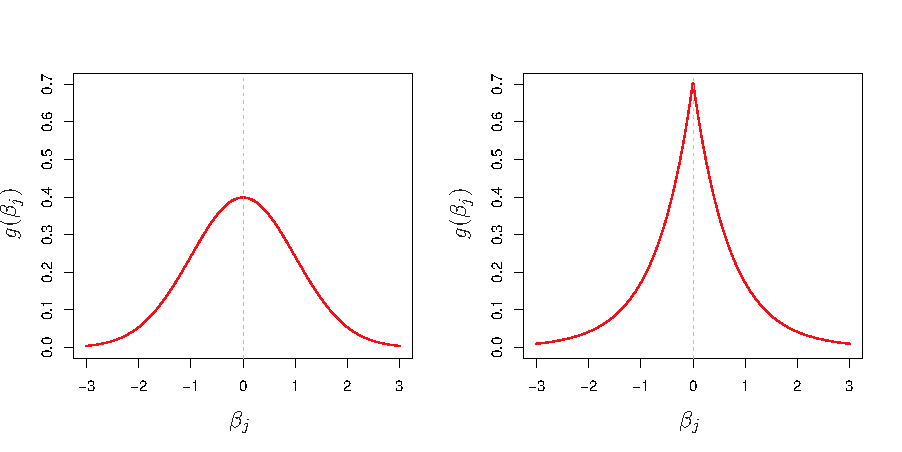
\includegraphics[scale=0.85]{../img/ISLR_ch6_fig11}
	\caption{Both Ridge and Lasso can be viewed as MAP estimators based on a Bayesian linear regression model. Whereas Ridge, at left, puts a normal prior on the regression coefficients, Lasso, at right, uses a Laplace prior, which has fatter tails and a taller peak at zero. This figure appears in Chapter 6 of James et al.\ (2013).}
	\label{fig:ridge_lasso_prior}
\end{figure}

When $p=2$, we can draw a picture of both the Ridge and Lasso problems in their ``budget constraint'' form. Both have the same objective function, which is proportional to the normal likelihood and describes a set of elliptical contours in $(\beta_1,\beta_2)$ -- space, centered at the MLE. Whereas Ridge has a circular constraint set, however, Lasso has a diamond-shaped one. Figure \ref{fig:ridge_lasso_constraint} shows how this difference in penalty functions leads to very different results. Sometimes the likelihood surface will hit a ``corner'' of the Lasso constraint set, leading to a zero coefficient estimate. In contrast, the Ridge constraint set has no corners and since it's circular there's nothing ``special'' about points on either axis.

\begin{figure}
	\centering
	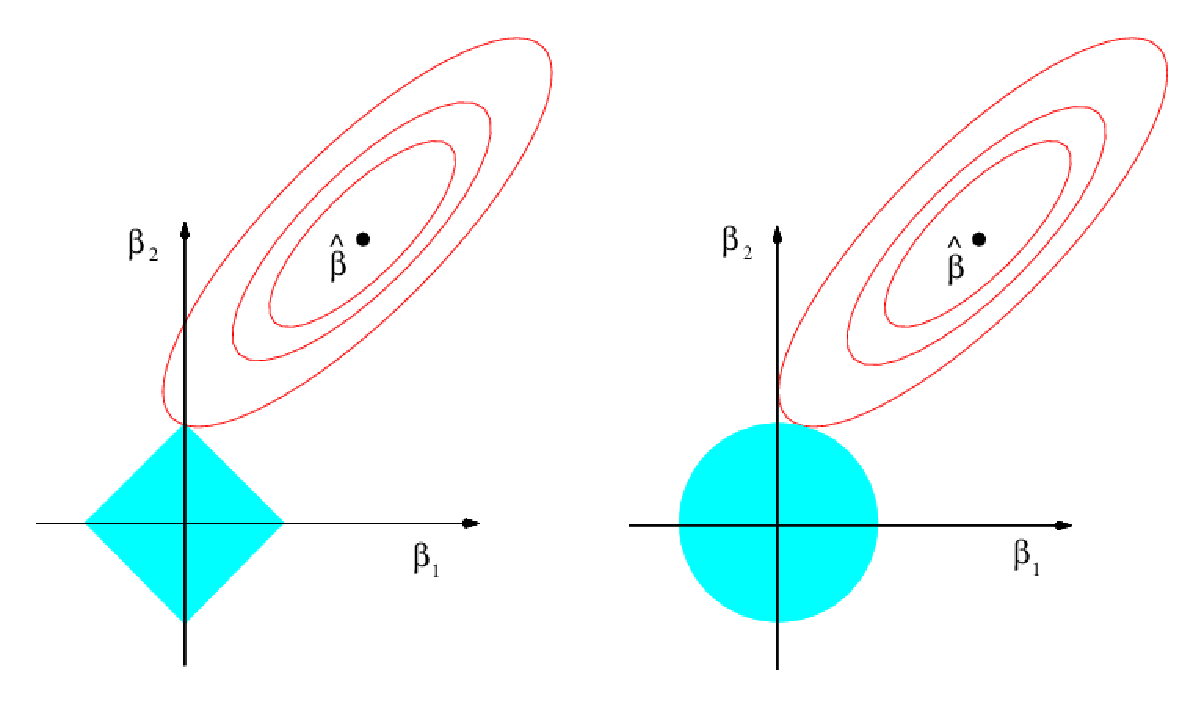
\includegraphics[scale=0.6]{../img/ISLR_ch6_fig7}
	\caption{In each panel $\widehat{\beta}$ denotes the MLE and the ellipses represent the contours of the likelihood. Both Lasso, at left, and Ridge, at right, shrink towards zero and away from the MLE. Because of its diamond-shaped constraint set, however, Lasso leads to a sparse solution, whereas Ridge does not. This figure appears in Chapter 6 of James et al (2013).}
	\label{fig:ridge_lasso_constraint}
\end{figure}

Yet another way to understand the difference between Ridge and Lasso is algebraically. For simplicity, and without loss of generality, suppose that $X$ is orthonormal. Another way of putting this is, suppose that we've replaced $X$ with its principal components. In this special case, it turns out that we can derive a closed form solution for Lasso. First we'll find the MLE. Since $X'X = I$, we have
	$$\widehat{\beta}_{MLE} = (X'X)^{-1}X'\textbf{y} = X'\textbf{y}$$
or written elementwise,
	$$\widehat{\beta}^{MLE}_j = \sum_{i=1}^n x_{ij}y_i$$
Similarly, for Ridge Regression we have
	$$\widehat{\beta}_{Ridge} =\left(X'X + \lambda I_p \right)^{-1}X'y = \left(I_p + \lambda I_p \right)^{-1} \widehat{\beta}_{MLE}$$
hence
	$$\widehat{\beta}^{Ridge}_j =  \left(\frac{1}{1+\lambda}\right)\widehat{\beta}^{MLE}_j$$
The calculations for Lasso are a bit more involved since there is no closed-form solution. We're trying to solve
	$$\underset{\beta}{\arg \min} (\mathbf{y}  - X\beta)' (\mathbf{y} - X\beta) + \lambda \left| \left| \beta\right| \right|_1$$
Now using $X'X = I$ along with $\widehat{\beta}_{MLE} = X'\textbf{y}$, we can expand the first term as
	\begin{eqnarray*}
		 (\mathbf{y}  - X\beta)' (\mathbf{y} - X\beta) &=& \mathbf{y}'\mathbf{y} - 2\beta' X' \mathbf{y} + \beta' X'X \beta \\
		 	&=& (\mbox{constant}) - 2\beta' \widehat{\beta}_{MLE} + \beta'\beta
	\end{eqnarray*}
Thus, for the case of orthonormal regressors we have:
\begin{eqnarray*}
	\widehat{\beta}_{Lasso} &=& \underset{\beta}{\arg \min} (\beta'\beta - 2\beta' \widehat{\beta}_{MLE})  +  \lambda \left| \left| \beta\right| \right|_1\\
		&=& \underset{\beta}{\arg \min}  \sum_{j=1}^p \left(\beta_j^2 - 2 \beta_j \widehat{\beta}^{MLE}_j + \lambda\left|\beta_j \right|\right)
\end{eqnarray*}
Here's the key: because the regressors are orthonormal, the optimization problem has been ``de-coupled.'' Since each $\beta_j$ only appears in one term of the sum, we can solve the overall optimization problem by solving $p$ \emph{completely independent} optimization problems:
	$$\widehat{\beta}^{Lasso}_j = \underset{\beta_j}{\arg \min} \left(\beta_j^2 - 2 \beta_j \widehat{\beta}^{MLE}_j + \lambda\left|\beta_j \right|\right)$$
Each of these $p$ objective functions has three terms. The first and third are always positive: they depend only on the absolute magnitude of $\beta_j$. In contrast, the second term could be either positive or negative depending on the signs of $\widehat{\beta}^{MLE}_j$ and $\beta_j$. Now, $\widehat{\beta}^{MLE}_j$ is outside our control: it's simply a function of the data. And whatever the \emph{magnitude} of $\beta_j$ changing its sign will not effect either $\beta_j^2$ or $\lambda|\beta_j|$. It follows that since we want to \emph{minimize} the criterion, we should \emph{match} the sign of $\beta_j$ to that of $\widehat{\beta}^{MLE}_j$. This ensures that the second term is negative. Accordingly, we consider two cases. 

\paragraph{Case I: $\widehat{\beta}^{MLE}_j >0$} As explained above we need to match the sign of $\beta_j$ to that of the MLE. Thus, we must have $\beta_j > 0$. Since $\beta_j >0$, it follows that $|\beta_j| = \beta_j$ and the problem becomes
	$$\widehat{\beta}^{Lasso}_j = \underset{\beta_j}{\arg \min} \; \beta_j^2 - 2 \beta_j \widehat{\beta}^{MLE}_j + \lambda\beta_j$$
Now that that pesky absolute value is gone, this is a straightforward calculus problem. The first order condition is $2\beta_j + \lambda = 2 \widehat{\beta}^{MLE}_j$. Solving, we have
	$$\beta_j = \widehat{\beta}^{MLE}_j - \frac{\lambda}{2}$$
But we're not quite done: we need $\beta_j > 0$ but the preceding expression will give a \emph{negative} value for $\beta_j$ if $\lambda$ is big enough. To keep this from happening, our corner solution must be to set $\beta_j = 0$ in this case. In other words, we have
	$$\widehat{\beta}^{Lasso}_j = \left(\widehat{\beta}^{MLE}_j - \frac{\lambda}{2} \right)_+ = \mbox{sign}\left(\widehat{\beta}^{MLE}_j \right)\left(\left| \widehat{\beta}^{MLE}_j\right| - \frac{\lambda}{2} \right)_+$$

\paragraph{Case II: $\widehat{\beta}^{MLE}_j \leq 0$} In this case, we must have $\beta_j \leq 0$ to match the sign of the MLE. It follows that $|\beta_j| = -\beta_j$ so the problem becomes
$$\widehat{\beta}^{Lasso}_j = \underset{\beta_j}{\arg \min} \; \beta_j^2 - 2 \beta_j \widehat{\beta}^{MLE}_j - \lambda\beta_j$$
The first order condition is $2\beta_j = 2\widehat{\beta}^{MLE}_j +\lambda$. Solving,
	$$\widehat{\beta}_j = \widehat{\beta}^{MLE}_j + \frac{\lambda}{2}$$
In this case we need $\beta_j <0$, just like $\widehat{\beta}^{MLE}_j$. But if $\lambda$ is sufficiently large, this requirement will be violated. To keep this from happening, our corner solution is, again, $\beta_j = 0$. We can express this as 
	$$\widehat{\beta}^{Lasso}_j =\mbox{sign}\left(\widehat{\beta}^{MLE}_j \right)\left(\left| \widehat{\beta}^{MLE}_j\right| - \frac{\lambda}{2} \right)_+$$
Hooray! We got the same answer in each case! To summarize, provided that $X$ is orthonormal, the Ridge and Lasso estimators are as follows:
	\begin{eqnarray*}
		\widehat{\beta}^{Ridge}_j &=&  \left(\frac{1}{1+\lambda}\right)\widehat{\beta}^{MLE}_j\\
		\widehat{\beta}^{Lasso}_j &=&\mbox{sign}\left(\widehat{\beta}^{MLE}_j \right)\left(\left| \widehat{\beta}^{MLE}_j\right| - \frac{\lambda}{2} \right)_+
	\end{eqnarray*}
Figure \ref{fig:ridge_lasso_shrink} depicts the difference between these two procedures. Whereas Ridge shrinks each element of $\widehat{\beta}_{MLE}$ by the same \emph{proportion}, namely $1/(1+\lambda)$, Lasso sets any elements of $\widehat{\beta}_{MLE}$ that are less than $\lambda/2$ to zero and \emph{translates} all other elements by a constant distance $\lambda/2$. 



\begin{figure}
	\centering
	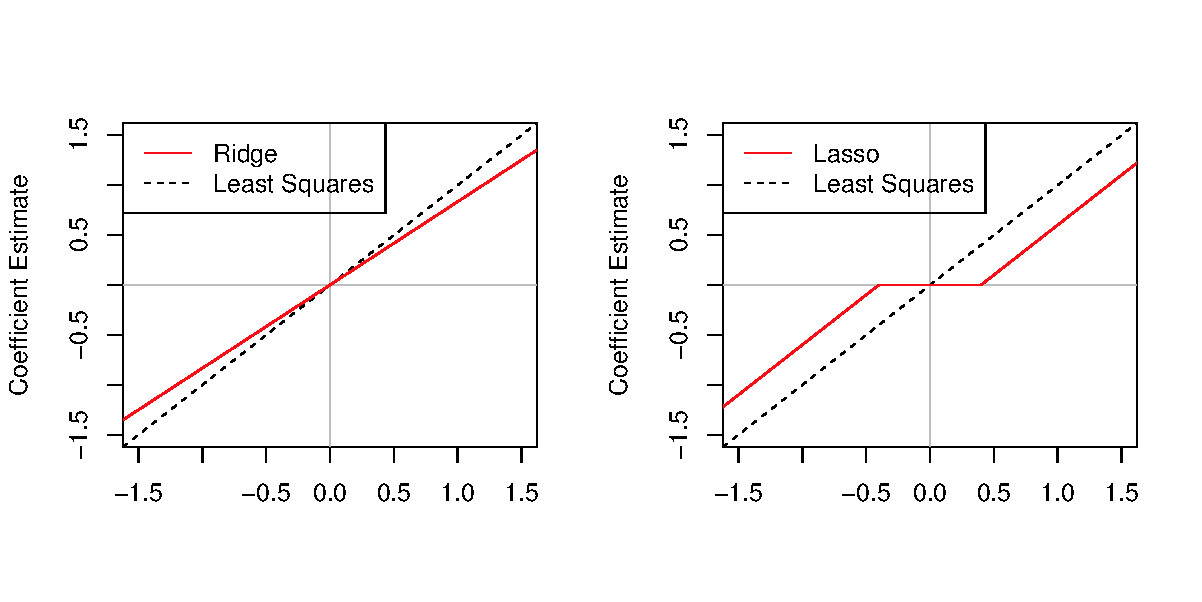
\includegraphics[scale=0.7]{../img/ISLR_ch6_fig10}
	\caption{These plots illustrate Ridge and Lasso shrinkage for the special case of orthonormal regressors. The horizontal axis in each plot is the MLE, while the vertical axis is the shrinkage estimator. Ridge appears at left and Lasso at right. The dashed 45-degree line in each plot corresponds to zero shrinkage. This figure appears in Chapter 6 of James et al (2013).}
	\label{fig:ridge_lasso_shrink}
\end{figure}

\subsection{Effective Degrees of Freedom for Lasso}
For a given value of $\lambda$ how complex is the corresponding Ridge fit compared to the Lasso fit? Is there a way for us to express these very different procedures in common units? We argued above that a reasonable measure of the complexity of Ridge Regression by $H(\lambda) = \mbox{trace}\left\{ X(X'X + \lambda I_p)^{-1} X'\right\}$. Since Lasso doesn't, in general, have a closed form it's not immediately clear what the appropriate analogy should be. It turns out (Zou, Hastie \& Tibshirani; 2007) that the the \emph{number of nonzero fitted coefficients} provides an unbiased estimator of effective degrees of freedom for Lasso. 

A cautionary note: two recent papers suggest that there are some complications in the analogy by which ``effective degrees of freedom'' in regularized regression are compared to parameter counts in ordinary regression. I haven't had a chance to look at these in detail yet, so if you're particularly keen you should write up a nice summary and send it to me! The papers are: Kaufman \& Rosset (2013) and Janson, Fithian \& Hastie (2013).

\subsection{How to Choose $\lambda$ for LASSO?}
Unlike Ridge, there's no computational shortcut for leave-one-out cross-validation that we can apply to Lasso. We can still use this procedure, but we have to do it the hard way. Of course we could also use $k$-fold cross-validation. But what about those model selection criteria we studied earlier in the semester? Is it possible to say anything about AIC, AIC$_C$, BIC, and $C_p$ in the context of Lasso estimation? The answer turns out to be \emph{yes} and many familiar properties carry over. Flynn, Hurvich and Simonoff (2013) show that the natural extensions of AIC, AIC$_C$ and $C_p$ to Lasso, using the effective degrees of freedom in place of the number of parameters, are asymptotically efficient. In a simulation study, they find that AIC, BIC and $C_p$ sometimes select values of $\lambda$ that are far too small: they ``catastrophically overfit.'' In contrast, AIC$_C$ performs well, just as it did in the case of ordinary linear regression. 

There is also a literature on the appropriate choice of $\lamba$ in settings where we hope to use Lasso to carry out variable selection. See the book \emph{Statistics for High-Dimensional Data} by B\"{u}hlmann and van de Geer (2011) for details and further references.


\subsection{Elastic Net}
There are arguments in favor of Ridge, and there are arguments in favor of Lasso. So why not try combining them? This is precisely the idea behind the so-called \emph{elastic net}. Rather than an $L_1$ or squared $L_2$-norm penalty, the elastic net uses
	$$\lambda \sum_{i=1}^p \left(\alpha \beta_j^2 + (1-\alpha)|\beta_j| \right)$$
The tuning parameter $\alpha$ controls ``how close'' the elastic net is to Ridge Regression. When $\alpha = 1$, we have Ridge. When $\alpha = 0$ we have Lasso. For any value in between, we have a combination of the two. For more on the elastic net, see Murphy (2013; Section 13.5.3).

% \subsection{Group LASSO}

% \subsection{Fused LASSO}

% \subsection{Inference for LASSO}
% All of this regularized linear regression stuff sounds great: it's computationally efficient and helps us make more reasonable predictions in a ``data-rich'' environment. But what if we want to carry out \emph{inference} for these models? Is there a simple way to proceed? 

% One option is go Bayesian: as long as we can sample from the posterior, we can construct credible intervals for any quantity of interest. Indeed, if we follow Park \& Casella and put a hyper-prior on ... we can even take uncertainty in the choose of smoothing parameter into account by integrating it out! 

% Things are much more complicated for Frequentists.

% Could go Bayesian. For a Frequentist, this is a very hard problem. A couple of recent papers, including Belloni et al.

\subsection{The Bayesian Lasso}
As mentioned above, the Lasso can be viewed as the MAP estimator from a Bayesian regression model with a Laplace prior, treating the error variance as known. The posterior mode, however, is a somewhat less than ideal summary. If forced to summarize a posterior using a single number we'd typically be much more comfortable with the mean or median. Park and Casella (2008) propose fully Bayesian version of the Lasso using a conditional Laplace prior for $\beta$ and a noninformative, scale-invariant prior for the error variance $\sigma^2$. Using the marginal likelihood to select $\lambda$, the posterior mean provides an estimator that is not exactly sparse, but appears to represent a compromise between Ridge and Lasso. By writing the Laplace distribution as a exponential scale mixture of normals, they show how to Gibbs sample the model and additionally consider inference and hyperpriors for $\lambda$.


\section{Shrinkage Estimation Using R}
Chapter 6 of James et al.\ (2013) ends with three ``Labs'' illustrating how to carry out various model selection and shrinkage procedures in R. The second and third of these contain Ridge Regression, Lasso, and PCR. There are some errors in the code as it appears in the book, so I've put together a corrected version with extensive comments called \texttt{ISLR\_ch6\_lab.R} and posted it in the GitHub repository for this class: \url{https://github.com/fditraglia/econ722}. This code makes heavy use of the excellent \texttt{GLMNET} package for R which is documented in Friedman, Hastie \& Tibshirani (2010). If you want to do your calculations using Matlab I'm afraid I can't offer you any guidance on the appropriate packages but if you send me some details, I'll include them in future versions of this document.
